\documentclass{beamer}
\usepackage{amsmath}
\usepackage{graphicx}

%% ===========================================
%% ===========================================
\title{\huge Martrix Analysis}
\author{Gunasekhar and Dileep Chandra}
\institute{IITH}
\date{\today}

%% ===========================================
%% ===========================================
\begin{document}


\begin{frame}[plain]
    \titlepage
\end{frame}
%% ===========================================
%% ===========================================



%% ===========================================
%% ===========================================
%	PRESENTATION SLIDES
%% ===========================================
%% ===========================================

%% ===========================================
%% ===========================================
\section{First Section} % Sections can be created in order to organize your presentation into discrete blocks, all sections and subsections are automatically printed in the table of contents as an overview of the talk
%% ===========================================
%% ===========================================

\subsection{Subsection Example} % A subsection can be created just before a set of slides with a common theme to further break down your presentation into chunks

%% ===========================================
%% ===========================================

\begin{frame}
\frametitle{Question:2}
A circle passes through the point (2,3) and (4,5) If the centre lies on the line (-1 4)X +3=0,then find the radius of the circle.
\end{frame}

%% ===========================================
%% ===========================================

\begin{frame}
\frametitle{Matrix Transformation}
\begin{itemize}
\item Circle equation:$(X-C)^T(X-C)=R^2$
\item $X^TX-2X^TC=R^2-C^TC$
 Since A(2,3),B(4,5) lie on circle
\item $A^TA-2A^TC=R^2-C^TC$ and $B^TB-2B^TC=R^2-C^TC$
\item $A^TA-2A^TC=B^TB-2B^TC$ 
\item so C must lie on line $(A-B)^TC=(A^TA-B^TB)/2$
\item also given c lies on 
\begin{equation}
[-1\ 4]X=-3
\end{equation}
\item C is the intersection point of above two lines
\end{itemize}
\end{frame}

%% ===========================================
%% ===========================================
\begin{frame}
\frametitle{Figure}
\begin{figure}[htp]
\centering
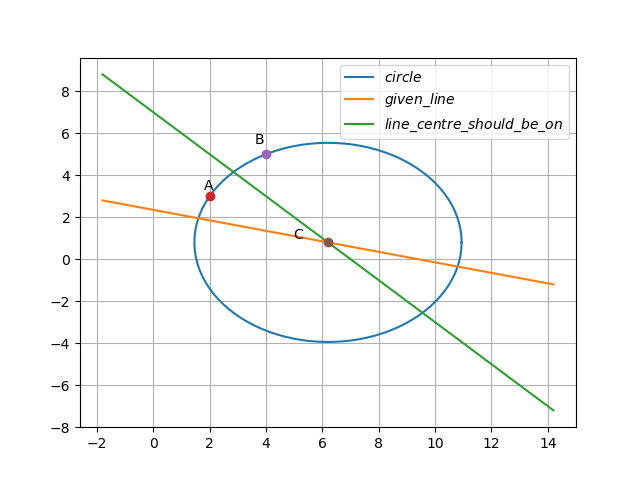
\includegraphics[width=10cm]{figure}
\caption{graph}
\label{fig:graph}
\end{figure}
\end{frame}
\begin{frame}
\frametitle{Solution}
\begin{itemize}
\item $((A-B)^T)C=(||A||^2-||B||^2)/2$        
\item $((A-B)^T)C=(3.605^2-6.403^2)/2$
\item $((A-B)^T)C=(13-41)/2$
\item $((A-B)^T)C=-14$
\begin{equation}
    [-2\ -2]C=-14
\end{equation}
\item from (1) and (2)\\
\item $(N^T)C=P$\\
\begin{gather}
\begin{bmatrix}
    -1 & 4 \\
    -2 & -2 
\end{bmatrix}
C=\begin{bmatrix}
    -3\\
    -14
\end{bmatrix}
\end{gather}
\begin{gather}
C=
\begin{bmatrix}
    -1/5 & -2/5 \\
    1/5 & -1/10 
\end{bmatrix}
\begin{bmatrix}
    -3\\
    -14
\end{bmatrix}
\end{gather}
\item so C=[+6.2\  +0.8]
\end{itemize}
\end{frame}

\begin{frame}
\frametitle{Conclusion}
\begin{itemize}
\item From solving we get C=[+6.2\ +0.8]
\item $Radius=|C-A|=|C-B|$
\item Radius=4.741307
\end{itemize}
\end{frame}


\begin{frame}
\Huge{\centerline{The End}}
\end{frame}

\end{document}